\chapter{Implementacja}
\section{Wybrane narzędzia i technologie}
\subsection{Java}

\begin{figure}[!htbp]
    \centering
    
\includegraphics[width=0.2\textwidth]{images/javaLogo.png}
    \caption{Oficjalne logo języka Java}
    \label{fig:enter-label}
\end{figure}

Java jest to szeroko stosowany obiektowy język programowania i platforma oprogramowania, która działa na miliardach urządzeń. Zasady oraz składnia języka zostały oparte na językach \acronym{C} i \acronym{C++}. Java powstała aby udoskonalić i naprawić wiele błędnych konceptów wprowadzonych przez te języki. Jedną z głównych zalet tworzenia oprogramowania w Javie jest jej przenoszalność. Po napisaniu kodu programu na jednym urządzeniu można go łatwo przenieść na inne urządzenie o innej architekturze. Język ten został wynaleziony w 1995 roku przez Jamesa Goslinga z Sun Microsystems (później przejętego przez Oracle), główną ideą jego wynalezienia była możliwość, \definicja{"napisania raz, uruchomienia w dowolnym miejscu"}  (\english{write once, run anywhere}). Nowe i ulepszone narzędzia do tworzenia oprogramowania pojawiają się na rynku w nizwykłym tempie, wypierając dotychczasowe produkty, które kiedyś uważano za niezbędne. W świetle tej ciągłej rotacji, długowieczność Javy jest imponująca, prawie trzy dekady po jej stworzeniu, Java jest nadal najpopularniejszym językiem do tworzenia oprogramowania użytkowego\cite{javaIBM}\cite{javaDEV}.

Wszystkie języki programowania służą do komunikacji z maszynami. Sprzęt maszynowy reaguje tylko na komunikację elektroniczną. Języki programowania wysokiego poziomu, takie jak Java, działają jako pomost między językiem ludzkim a językiem sprzętu. Aby korzystać z języka Java programista musi mieć świadomość o dwóch poziomach abstrakcji pisanych programów: 

\begin{itemize}
    \item Język Java i \definicja{interfejsy \acronym{API} }(\english{application programming interface})
    \item Wirtualna maszyna Java \acronym{JVM} (\english{\termdef{Java Virtual Machine}})
\end{itemize}

Java definiuje składnię i semantykę języka. Obejmuje to podstawowe słownictwo i reguły używane do pisania algorytmów. 
Interfejsy API są ważnymi komponentami oprogramowania dołączonymi do platformy Java. Są to wstępnie napisane programy, które można podłączyć i odtworzyć istniejące funkcjonalności we własnym kodzie. Na przykład można użyć interfejsów API Java, aby uzyskać datę i godzinę, wykonać operacje matematyczne lub manipulować tekstem. Każdy kod aplikacji Java napisany przez programistę zazwyczaj łączy nowy i wcześniej istniejący kod z interfejsów API Java, bibliotek i frameworków\cite{frameworkDef}\cite{javaAmazon}\cite{javaDEV}.

Wirtualna maszyna Javy działa jako dodatkowa warstwa abstrakcji między platformą Java a sprzętem maszyny. Kod źródłowy Java może działać tylko na tych maszynach na których zainstalowano JVM. Kiedy po raz pierwszy opracowano języki programowania, dzieliły się one na dwie szerokie kategorie, w zależności od tego, w jaki sposób komunikowały się ze sprzętem: 

\begin{itemize}
    \item Kompilowany - program jest napisany w składni języka, a następnie kompilator tłumaczy cały kod na kod maszynowy. Skompilowany kod jest następnie uruchamiany na sprzęcie.
    \item Interpretowany - Dzięki interpreterom każda instrukcja kody wysokiego poziomu jest na bieżąco interpretowana na kod maszynowy. Napisane instrukcji są natychmiast uruchamiane przez sprzęt przed przejściem do następnej instrukcji
\end{itemize}

Język Java był pierwszym językiem, który połączył obie powyższe metody, przy użyciu JVM. Każdy plik programu jest najpierw kompilowany do kodu bajtowego (\english{bytecode}). Kod bajtowy Java może być uruchamiany tylko w maszynie JVM. Następnie JVM interpretuje kod bajtowy, aby uruchomić go na podstawowej platformie sprzętowej. Jeżeli aplikacja działa na komputerze z systemem Windows, maszyna JVM zinterpretuje ją dla systemu Windows. Natomiast jeżeli aplikacja uruchomiona jest na platformie open-source, takiej jak Linux, JVM zinterpretuje ją dla systemu Linux\cite{javaAmazon}\cite{javaDEV}.

\subsection{Maven}

\begin{figure}[!htbp]
    \centering
    
\includegraphics[width=0.5\textwidth]{images/mavenLogo.png}
    \caption{Logo programu Apache Maven\cite{mavenSite}.}
    \label{fig:enter-label}
\end{figure}

Maven słowo w języku jidysz oznacza gromadzenie wiedzy. Apache Maven to narzędzie do zarządzania projektami oprogramowania. Opiera się on na koncepcji modelu obiektu projektu (\acronym{POM} \english{Project Object Model}), Maven może zarządzać kompilacją, raportowaniem i dokumentacją projektu z centralnej informacji. Narzędzie to wykorzystywane jest do budowania i zarządzania dowolnym projektem opartym na Javie. Głównym źródłem informacji o projekcie jest plik \akronim{XML} (\english{Extensible Markup Language}) nazywany \acronym{POM}, w którym definiowana jest struktura projektu, sposób jego budowania oraz zależności jakie są wymagane do prawidłowego funkcjonowania programu. Maven podcza budowania aplikacji pobiera niezbędne biblioteki oraz inne zależności z globalnego repozytorium Maven Central.

\subsection{Spring boot}

\begin{figure}[!htbp]
    \centering
    
\includegraphics[width=0.5\textwidth]{images/springboot/springBootLogo.png}
    \caption{Logo frameworka Spring Boot \cite{springLogo}}
    \label{fig:enter-label}
\end{figure}


Spring boot jest jednym z najpopularniejszych frameworków języka Java wynalezionym przez Roda Johnsona w 2014 roku, który zapewnia funkcjonalność błyskawicznego wytwarzania aplikacji (\english{\definicja{Rapid Application Development \akronim{RAD}}}) polegającego na udostępnianiu programiście dużych możliwości prototypowania oraz dużego zestawu gotowych komponentów, narzędzi i modułów\cite{RADwiki}. Spring boot zbudowany jest na popularnym Java Spring Framework, aby zapewnić szybki dostęp do informacji podczas tworzenia projektu. Metodyka RAD jest dość łatwa do skonfigurowania i uruchomienia w internetowych i korporacyjnych aplikacjach przy użyciu języka Java. Najważniejszą rzeczą w tym frameworku jest jego prostota, do uruchomienia aplikacji wymagana jest minimalna konfiguracja, dzięki czemu tworzenie samodzielnych aplikacji opartych na Springu jest o wiele łatwiejsze\cite{springbootAnalysis}.

\subsubsection{Główne cechy Spring Boot Framework}

\begin{enumerate}
    \item Autokonfiguracja: Funkcja automatycznej konfiguracji Spring Boot automatycznie konfiguruje aplikację Spring na podstawie dodanych zależności. Na przykład, jeżeli została dołączona zależność spring-boot-starter-web, automatycznie zostaje skonfigurowany serwer Tomcat i Spring \acronym{MVC} (\english{Model-View-Controller})\cite{springbootFeatures}.
    \item Samodzielna aplikacja: Aplikacje Spring Boot mogą być uruchamiane jako samodzielne aplikacje Java. Jest to ułatwione dzięki osadzeniu serwera HTTP (takiego jak Tomcat, Jetty lub Undertow) bezpośrednio w aplikacji, co ułatwia jej wdrożenie\cite{springbootFeatures}.
    \item Funkcje gotowe do produkcji: Spring Boot zawiera kilka wbudowanych funkcji ułatwiających uruchamianie aplikacji w środowisku produkcyjnym. Obejmują one kontrole kondycji, metryki, monitorowanie aplikacji i konfigurację zewnętrzną\cite{springbootFeatures}.
    \item Konwencja ponad konfiguracją: Spring Boot kieruje się filozofią zapewniania rozsądnych wartości domyślnych, aby zminimalizować ilość wymaganej konfiguracji. Jednak nadal pozwala na zastąpienie tych domyślnych ustawień, gdy jest to konieczne\cite{springbootFeatures}.
    \item Rozwój mikrousług: Spring Boot jest szeroko stosowany do tworzenia mikrousług ze względu na jego lekki i modułowy charakter. Zapewnia wbudowane serwery, łatwą integrację ze środowiskami chmurowymi i wsparcie dla systemów rozproszonych\cite{springbootFeatures}.
    \item Startery Spring Boot: Startery to zestaw wygodnych deskryptorów zależności, które można dołączyć do aplikacji. Na przykład spring-boot-starter-data-jpa zawiera zależności do używania \acronym{JPA} (\english{Java Persistence \acronym{API}}) ze Spring Data\cite{springbootFeatures}.
    \item Wbudowane serwery: Spring Boot obsługuje wbudowane serwery, takie jak Tomcat, Jetty i Undertow, umożliwiając pakowanie aplikacji jako plików \acronym{JAR} (\english{Java Archive}) i uruchamianie ich niezależnie od zewnętrznych serwerów\cite{springbootFeatures}.
    \item Spring Initializr: Spring Initializr to narzędzie internetowe do szybkiego generowania struktury projektu Spring Boot. Pozwala programistom wybrać żądane zależności projektu i wygenerować szkielet projektu\cite{springbootFeatures}.
    \item Obszerna dokumentacja i wsparcie społeczności: Spring Boot jest dobrze udokumentowany i ma dużą i aktywną społeczność, która przyczynia się do jego ciągłego rozwoju i wsparcia\cite{springbootFeatures}.
    \item Korzystając ze Spring Boot, programiści mogą usprawnić tworzenie aplikacji opartych na Spring, wykorzystując potężne funkcje frameworka w celu zmniejszenia ilości standardowego kodu i wysiłku związanego z konfiguracją\cite{springbootFeatures}.
\end{enumerate}

\begin{figure}[!h]
    \centering
    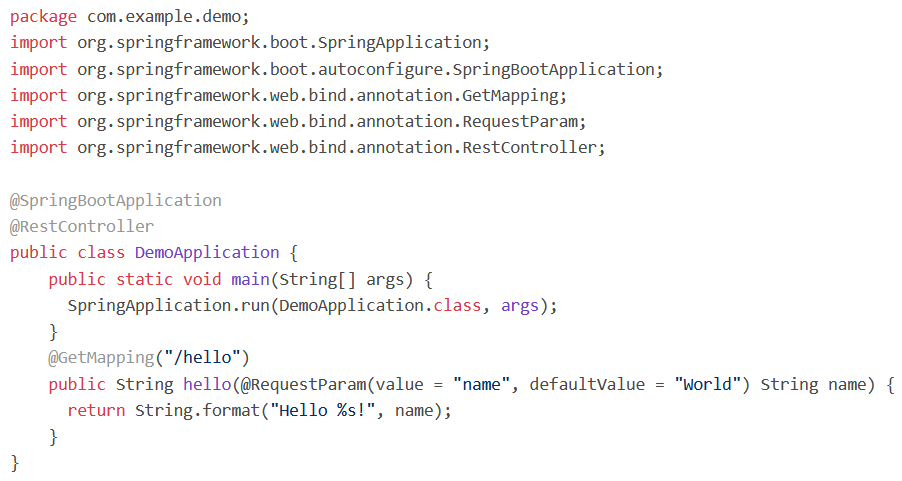
\includegraphics[width=0.8\textwidth]{images/springboot/exampleJavaSpringBootProgram.png}
    \caption{Przykładowy program java napisany z wykorzystaniem frameworku Springboot\cite{springJavaExampleProgram}}
    \label{fig:enter-label}
\end{figure}

Powyższy program składa się z głównej klasy aplikacji z adnotacją @SpringBootApplication, która wskazuje klasę konfiguracyjną, która deklaruje jedną lub więcej metod @Bean, a także uruchamia automatyczną konfigurację i skanowanie komponentów. Klasa DemoApplication zawiera główną metodę, która jest punktem wejścia aplikacji. Metoda SpringApplication.run uruchamia cały framework Spring.
Dodatkowo klasa jest opatrzona adnotacją @RestController, wskazującą, że jest to kontroler sieciowy, w którym każda metoda zwraca obiekt domeny zamiast widoku. Metoda hello jest mapowana do punktu końcowego /hello przy użyciu adnotacji @GetMapping, co pozwala jej obsługiwać żądania HTTP GET. Metoda ta przyjmuje nazwę parametru żądania z domyślną wartością „World” i zwraca wiadomość powitalną.

\subsection{Netflix Eureka}

test

\subsection{Docker}

\begin{figure}[!htbp]
    \centering
    
\includegraphics[width=0.5\textwidth]{images/Docker_logo.png}
    \caption{Logo marki Docker \cite{DockerMedia}}
    \label{fig:enter-label}
\end{figure}

\subsubsection{Docker Compose}
\subsection{Środowisko programistyczne}
\subsection{Insomnia}
\subsection{Logstash Logback Encoder}




\section{Elementy tworzonego systemu}

\subsection{Producent}
\subsection{Rejestr usług}
\subsection{Węzeł protokołu}
\subsubsection{Podsystem monitoringu producentów}
\subsubsection{Podsystem propozycji zasobów}

\section{Uruchomienie środowiska}